\section{When Does Readback Change the Outcome?}
\subsection{Re-encoding at a measured origin}
After the five-step override, direct copying succeeded on 22 of 48 Fetch layouts. Re-encoding the desired target from the measured hand succeeded on 41 of 48, matching the number of successful source demonstrations. It rescued ten push and nine pick-and-place trials without losing any or requesting the controller target. Figure~\ref{fig:fetch} shows one rescued push. Under force alone re-encoding lost one push that direct copying completed, even though across force trials the mean hand-path RMS error fell from 0.033 to 0.005\,mm. Improving hand tracking does not ensure the cube finishes closer to its goal.
\begin{figure}[t]
\centering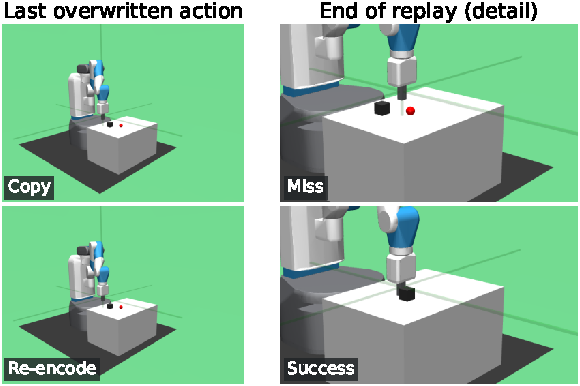
\includegraphics[width=\columnwidth]{figures/fetch-example.pdf}
\caption{Replay of the same FetchPush layout after five overwritten translations. At tick 14 the final overwrite occurs (left). At the last tick the cube is 134.4\,mm from the goal under direct copying and 23.3\,mm from it after re-encoding (right, enlarged). We show the lowest-index held-out push layout rescued by re-encoding.}\label{fig:fetch}
\end{figure}

\subsection{How much does Sawyer's hand already reveal?}
The clearest comparison holds the observer fixed and varies access to the internal target. On 36 fresh Sawyer layouts (12 per task), the hand-based observer recovered six trials lost by command history alone, with no losses. Reading on events while retaining command history recovered exactly the same six. Adding event reads to the hand-based observer changed none of the 144 paired terminal outcomes (Table~\ref{tab:observer}). The 123 extra reads reduced mean hand-path RMS error by 0.039\,mm (paired 95\% layout-bootstrap interval for the reduction, 0.012--0.068\,mm). Four push trials still failed with either observer branch.
\begin{table}[t]\centering
\caption{Sawyer policies on the same 36 layouts and four conditions per layout. Reads are total extra requests. RMS is the mean of per-episode hand-path errors.}\label{tab:observer}
\begin{tabular}{@{}lrrr@{}}\toprule
Origin estimate and read policy & Success & Reads & RMS (mm)\\\midrule
Command history only & 134/144 & 0 & 6.497\\
Command history + event & 140/144 & 112 & 2.734\\
Hand-based observer & 140/144 & 0 & 2.830\\
Observer + event & 140/144 & 123 & 2.790\\
Observer + gated fixed times & 140/144 & 32 & 2.829\\\bottomrule
\end{tabular}
\end{table}

Earlier schedule comparisons illustrate why the choice of baseline matters. With command history and hand feedback gain $k=0.5$, event and scheduled reads yielded 192/192 and 190/192 successes on push and pick-place, using 160 and 384 reads, respectively. The two event-only successes arose on a single pick-place layout, under the overwrite and combined conditions (Fig.~\ref{fig:sawyer}). The difference was 1.04 percentage points (95\% layout-bootstrap interval, 0.00--3.13). It fell short of the prespecified five-point gain with a positive lower confidence limit. The 96 drawer conditions agreed. At $k=0$, event reads succeeded on 192/192 compared with 166/192 for the scheduled reads. The larger difference applies to this weaker hand-feedback comparator.
\begin{figure}[t]
\centering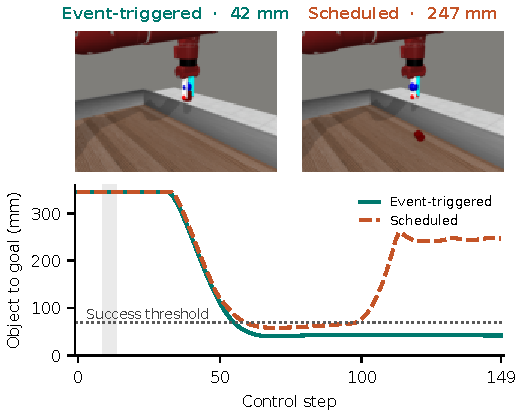
\includegraphics[width=\columnwidth]{figures/sawyer-case.pdf}
\caption{The single Sawyer pick-place layout accounting for both event-only successes against scheduled reads at $k=0.5$. During the overwrite trial both policies brought the object within 70\,mm of its goal. At the final step the event branch was 42.3\,mm away and the scheduled branch 246.7\,mm away.}\label{fig:sawyer}
\end{figure}

Checking the hand residual twice versus at every step on 36 fresh layouts gave 144/144 successes for both, with 60 versus 106 reads and 4.16 versus 3.14\,mm mean hand RMS. On a separate 36 layouts the rewrite guard~\eqref{eq:guard} admitted 658 of 12,474 proposals. Of these, 560 reached the setter, and each reduced squared write error as certified. Both guarded and unguarded branches succeeded on all 144 trials. The guard used more reads (125 versus 115) and had greater hand RMS (2.96 versus 2.64\,mm). Its guarantee is local to a delivered write.

On 24 further push and pick-place layouts, we timed overrides to begin six steps before or one step after the first pad--object contact in the source. The observer alone and a single read 0, 1, 2, 4 or 8 steps after the overwrite each achieved 48/48 across the two phases. Before the read, the mean origin error fell from 28.90\,mm at zero delay to 10.68\,mm at eight steps. The no-read and immediate-read hand RMS values were 8.02 and 7.95\,mm.

To test a trigger without access to the fault time, we compared two candidate commands computed from the available origin estimates. The policy could request once when their difference exceeded 2.5\,mm for two steps. On a separate 24-layout cohort, adding this trigger changed no terminal outcome relative to the zero-request observer. Both scored 96/96 with synchronous observations, 94/96 with a two-step delay, and 96/96 when the delayed interface also published the target every three steps. Under delay the 48 extra requests raised mean hand-path RMS from 4.429 to 4.504\,mm. The two failures without the periodic stream came from one pick-place layout.

\subsection{Changing the command origin on the same Panda}
To control for robot identity, we switched the native Cartesian controller of one simulated Panda between measured and accumulating origins in robosuite 1.5.2 (MuJoCo 3.3.7)~\cite{robosuite2020}. We used the same eight initial physical layouts in both modes and generated a clean source for each mode and layout. At 20\,Hz the source closed the gripper at step 60 and raised it at step 80. We overwrote five translations during descent (steps 35--39) or lift (80--84). One observer branch read once immediately after the scheduled override. This timing tests the effect of knowing the origin at that instant. Success required the cube center to finish more than 40\,mm above the table at step 120. All 16 sources succeeded. We retained all 192 replays, including failures.

After the descent override, direct copying failed on every layout in both modes. On the measured-origin controller, re-encoding from the current hand rescued all eight. On the accumulating controller, integration of submitted commands rescued none, whereas the hand-based observer and the observer with one read each rescued all eight. During lift every policy succeeded on all eight layouts. All terminal successes also held over the last 20 steps.
\begin{figure}[t]
\centering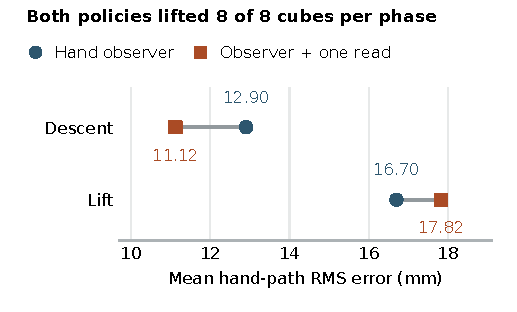
\includegraphics[width=\columnwidth]{figures/replay-comparison.pdf}
\caption{Paired replays on the accumulating Panda controller. A read after the descent override reduced mean hand-path RMS error from 12.90 to 11.12\,mm. During lift it increased the error from 16.70 to 17.82\,mm. Both observer policies lifted the cube on all eight layouts in each phase.}\label{fig:panda}
\end{figure}

The effect on the written target differed by phase. A descent read changed the next target by 24.13\,mm on average. During lift it corrected a mean origin estimate error of 120.32\,mm but changed the next target by only 0.026\,mm. Both policies had already requested maximum upward translation on every layout. Subsequent hand trajectories could still diverge (Fig.~\ref{fig:panda}).

\subsection{Three rescues with coarse hand feedback}
With two-step observation latency, unrounded and 1\,mm hand observations yielded 94/96 Sawyer successes with and without an event read on 24 push and pick-place layouts. On a 5\,mm grid the event policy achieved 94/96 versus 91/96 for the observer alone. All three extra successes came from two push layouts. The policy requested on all 96 development episodes, including all 24 clean episodes.

On 24 new layouts with the 5\,mm grid, the zero-read, event, fixed-time and permuted-time policies each succeeded on 96/96. They used 0, 94, 96 and 96 reads and had mean hand RMS errors of 6.409, 6.227, 6.293 and 6.399\,mm, respectively. The development rescues did not recur (Fig.~\ref{fig:confirm}). The ceiling in the new cohort limits inference about rarer conditions in which a read might rescue contact.

\begin{figure}[t]
\centering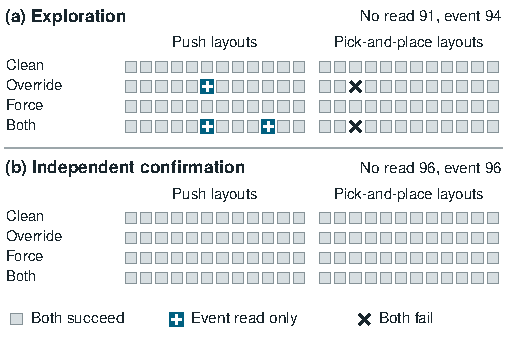
\includegraphics[width=\columnwidth]{figures/sawyer-confirmation.pdf}
\caption{Paired terminal outcomes with 5\,mm Sawyer hand observations. Each column is one layout and each row one intervention. Three event-only successes came from two development layouts. The four frozen policies each succeeded on every confirmation trial.}\label{fig:confirm}
\end{figure}
